\chapter{Marco teórico}
\label{Chapter1}
\lhead{Capítulo 1. \emph{Marco teórico}}

Este capítulo presenta brevemente los conceptos teóricos básicos para el
desarrollo de este trabajo. Primero se explican los fundamentos de la
planificación automática, área que provee un formalismo al cual se pueden
traducir problemas de decisión. Luego, se define la disciplina de complejidad
descriptiva, que determina la clase de complejidad computacional de distintos
fragmentos de lógica de segundo orden según su expresividad.
Finalmente, se explican dos ejemplos de problemas NP fácilmente modelables
con el formalismo lógico propuesto.

\section{Planificación automática}
La planificación automática es un campo de investigación dentro de la Inteligencia
Artificial. Su enfoque se basa en descubrir una secuencia de acciones a seguir para
lograr un objetivo concreto \citep{russell:book}. En este trabajo se manejará
la concepción \textbf{clásica} de planificación, en la cual todas las acciones
tienen una consecuencia determinística y observable en ambientes estáticos (es
decir, que sólo cambian con el resultado de las acciones aplicadas).

\cite{fikes:strips} fueron pioneros en el área de planificación con su sistema
STRIPS (\textit{Stanford Research
Institute Problem Solver}).

Los investigadores de esta área han diseñado una representación compacta para
expresar problemas de planificación de cualquier dominio, llamado PDDL
(\textit{Planning Domain Definition Language}).
En este trabajo se considera el fragmento más simple de PDDL, que es
equivalente a STRIPS.
Este fragmento describe todo lo necesario
para especificar un problema: el estado inicial, las acciones posibles con sus
precondiciones y efectos, y los estados meta.

La Definición \ref{definicion_planificacion} presenta de manera formal qué es
un problema de planificación. Los párrafos siguientes contienen una explicación
intuitiva del problema.

\begin{definition}
\label{definicion_planificacion}
Matemáticamente, se define un problema de planificación STRIPS como $P = \tup{C, A, I,
F}$, donde: 
\begin{itemize} 
\item $C$ es un conjunto de \textbf{condiciones} o variables proposicionales.
\item $A$ es un conjunto de \textbf{acciones}. Cada acción $a$ es
una tupla $a = \tup{pre, adds, deletes}$ que contiene el conjunto de
precondiciones (condiciones que deben ser ciertas para poder aplicar la acción)
y el conjunto de efectos positivos (\textit{adds}) y negativos (\textit{deletes}) que causa la
aplicación de la acción.
\item $I\subseteq C$ es el \textbf{estado inicial}. Los estados son
especificados por el conjunto de condiciones que son verdaderas en ellos, las
demás condiciones se suponen falsas. Esto se llama la suposición del
\textbf{mundo cerrado} \citep{russell:book}.
\item $F\subseteq C$ describe los \textbf{estados finales} o meta.
\end{itemize}
\end{definition}

Cada estado se representa con un conjunto de proposiciones, representadas
internamente como variables proposicionales pero expresadas frecuentemente como
símbolos relacionales instanciados.
Por ejemplo, en un problema de
planificación canónico llamado \textit{mundo de bloques}, una mano
robótica intenta apilar bloques enumerados de manera de que todos los bloques
estén en una sola pila ordenados de forma ascendente. Cada bloque puede tener a
lo sumo un bloque encima suyo, y la mano sólo puede cargar un bloque a la vez.
En este caso, proposiciones válidas que pueden ser parte de un estado son,
por ejemplo,
\texttt{manoVacía}, \texttt{sobreMesa(bloque0)}, \texttt{sobreMesa(bloque1)},
\texttt{libre(bloque0),
\texttt{libre(bloque1)}}.
La Figura \ref{blocksworld_inicial} ilustra un estado cuyas únicas
proposiciones ciertas son estas mencionadas anteriormente.
\begin{figure}[h!]
\centering
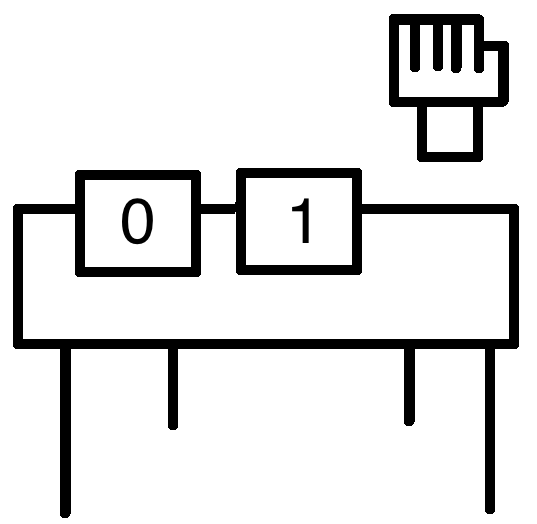
\includegraphics[width=0.4\textwidth]{figuras/blocksworld_inicial.png}
\caption[Ejemplo de estado inicial en \textit{mundo de bloques}]{Posible estado de un problema en \textit{mundo de bloques}.}
\label{blocksworld_inicial}
\end{figure}

Una acción en PDDL especifica qué debe ser cierto sobre el estado actual para
que la acción sea aplicable. 
Este conjunto comprende las \textbf{precondiciones}. Asimismo,
la acción declara qué proposiciones en el mundo cambian cuando es aplicada,
lo cual constituye sus \textbf{efectos}. Para una notación
simplificada, PDDL permite la utilización de \textbf{parámetros} en los
símbolos relacionales que describen sus precondiciones y efectos. Estos
parámetros pueden ser instanciados con cualquier objeto. Volviendo al
ejemplo anterior, un conjunto de acciones podría ser:
\begin{Verbatim}[commandchars=\\\{\},
codes={\catcode`$=3\catcode`^=7}]
(:action recoger_bloque
    :parameters (?b)
    :precondition (and (manoVacía) (libre ?b))
    :effect (and (enMano ?b) (not (manoVacía)) (not (sobreMesa ?b)))
)

(:action colocar_sobre
    :parameters (?b1 ?b2)
    :precondition (and (enMano ?b1) (libre ?b2))
    :effect (and (sobre ?b1 ?b2) (manoVacía) (not (enMano ?b1))
            (not (libre ?b2)))
)
\end{Verbatim}

Teniendo en cuenta esta especificación, el lector puede hacer el ejercicio de
generar una secuencia ordenada de acciones que resuelva este ejemplo
concreto, es decir, que conduzca desde el estado ilustrado en la Figura
\ref{blocksworld_inicial} hasta un estado en el cual los bloques estén ``apilados en
orden''. La solución se presenta a continuación. Como es costumbre, sólo se
mencionan las proposiciones verdaderas en cada estado. Se ha coloreado de azul
las nuevas proposiciones que han resultado de aplicar una acción
(\textit{adds}), y de rojo a las proposiciones que dejaron de ser ciertas en el
siguiente estado producto de la acción aplicada (\textit{deletes}).
\begin{Verbatim}[commandchars=\\\{\},
codes={\catcode`$=3\catcode`^=7}]
estado: \{sobreMesa(bloque0), {\color{red} sobreMesa(bloque1)},
         libre(bloque0), libre(bloque1), {\color{red} manoVacía}\}
\textit{acción: recoger_bloque(bloque1)}
estado: \{{\color{blue}enMano(bloque1)}, sobreMesa(bloque0),
        {\color{red} libre(bloque0)}, libre(bloque1)\}
\textit{acción: colocar_sobre(bloque1, bloque0)}
estado: \{{\color{blue}sobre(bloque1, bloque0)}, sobreMesa(bloque0),
          {\color{blue}manoVacía}, libre(bloque1)\}
\end{Verbatim}

La Figura \ref{blocksworld_final} es una representación de este estado final.

\begin{figure}[h!]
\centering
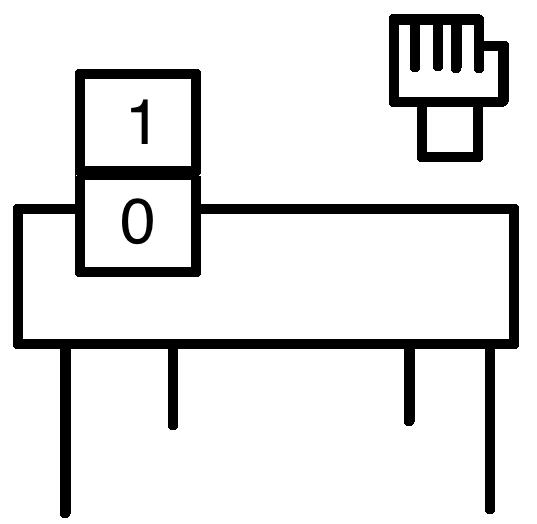
\includegraphics[width=0.4\textwidth]{figuras/blocksworld_final.png}
\caption[Estado final en \textit{mundo de bloques}]{Estado final para un problema en \textit{mundo de bloques},
luego de aplicar una secuencia de acciones al estado en la Figura
\ref{blocksworld_inicial}}
\label{blocksworld_final}
\end{figure}

En resumen, un \textbf{problema de planificación} es expresado utilizando
el lenguaje PDDL, que especifica su \textbf{estado inicial}, \textbf{acciones}
(precondiciones y efectos de cada una) y los \textbf{estados finales}.
Un \textbf{plan} es una secuencia ordenada de acciones que resuelve el problema
de planificación.

Cuando se busca resolver varias instancias de un problema general se suelen
agrupar los problemas de planificación en dominios. Dos problemas del mismo
dominio comparten el mismo conjunto de acciones, mas no necesariamente el
estado inicial o los estados meta. Por esto se dice que \textit{mundo de bloques}
es un \textbf{dominio de planificación}, y el término \textbf{problema} se refiere a
una instancia particular con estados inicial y final definidos, en
el cual pueden utilizarse las acciones del dominio al que pertenece.


Un problema de planificación en PDDL es un par $\tup{\domain,\instance}$ con
una descripción de un dominio y una instancia en el lenguaje PDDL
\citep{mcdermott:pddl,fox:pddl}.
\subsection{Complejidad en planificación}
\label{complejidad_planificacion}
Sea PLANSAT el problema de decisión que pregunta si existe un plan que
resuelve un problema de planificación dado. Según el formalismo que se ha definido
en la sección anterior,
PLANSAT es \textbf{decidible} porque el número de estados es finito:
un algoritmo basado en búsqueda desde el estado inicial que aplique
todas las acciones posibles en cada estado acabará examinando todo el espacio y
determinando si existe tal plan.

PLANSAT pertenece a la clase de complejidad PSPACE
\citep{bylander:plan-complexity}.
PSPACE es la clase de problemas que pueden ser resueltos por una máquina de
Turing determinística con una cantidad polinomial (en $n$, donde $n$ es el
tamaño del problema) de espacio en memoria. Los problemas PSPACE son, en
general, más difíciles de resolver que los problemas NP, los cuales a su vez
son problemas combinatorios complejos para los cuales se cree que no existen
soluciones generales eficientes. Como en muchos otros dominios de inteligencia
artificial, los planificadores dependen de
heurísticas de búsqueda para dar con las soluciones a problemas pequeños en un 
período de tiempo razonable.

Una restricción interesante a PLANSAT es no permitir efectos negativos en las
acciones. Si este es el caso, cualquier predicado instanciado que se haya 
agregado permanece cierto durante todo el plan, de modo que no es necesario
que el operador instanciado sea aplicado más de una vez.
Esto tiene como consecuencia que PLANSAT sin efectos 
negativos pertenezca a la clase NP \citep{ghallab:book}.

\section{Complejidad Descriptiva}
La Teoría de Complejidad Descriptiva (TCD) es un área de investigación en la
intersección entre matemáticas y las ciencias de la computación 
que estudia la teoría de complejidad desde un punto de vista matemático, 
sin utilizar modelos de computación como máquinas de Turing. La TCD surgió
cuando se demostró que la clase de complejidad NP corresponde
exactamente con la clase de problemas expresables en lógica de segundo orden
existencial \citep{fagin:spectra}. En los últimos años se ha establecido una
correspondencia entre las clases de complejidad más importantes y lenguajes
lógicos con distintos niveles de expresividad \citep{immerman:book}. En esta
sección se describen los elementos sintácticos de estos lenguajes, repasando
conceptos relevantes de la lógica, y se explica la interpretación formal de
las fórmulas construidas con estos lenguajes.

\subsection{Lenguajes}
Cada lenguaje lógico está construido a partir de un conjunto de símbolos, o
\textbf{vocabulario}.
El vocabulario se suele dividir en símbolos lógicos puros como `$\land$',
`$\exists$', etc., símbolos de puntuación como `$($' y `$)$', símbolos
relacionales, símbolos funcionales y constantes. Los símbolos lógicos y de
puntuación pertenecen a todos los lenguajes, mientras que los símbolos
relacionales, funcionales y constantes varían de un lenguaje a otro. De modo
que es conveniente definir la firma de un lenguaje como el conjunto finito de
relaciones, funciones y constantes permitidas en las fórmulas. Las firmas son
denotadas por tuplas como $\sigma=\tup{P^1,Q^2,f^1,A,B}$, que contiene dos
símbolos relacionales $P$ y $Q$ de aridades 1 y 2, respectivamente, un símbolo
funcional $f$ de aridad 1, y dos constantes $A$ y $B$.

Los símbolos funcionales de la forma $f(x) = y$ pueden representarse con una
tupla de la relación $F(x, y)$, en la que se expresa que $y$ es la imagen de
$x$, siempre y cuando se agreguen restricciones sobre $x$ y $y$ que expresen
que $f$ es una función.
Por esta razón se omiten los símbolos funcionales en lo sucesivo.

\subsubsection{Lógica de segundo orden}
Se denota con $\LPO(\sigma)$ y $\LSO(\sigma)$ a los conjuntos de todas las
fórmulas de lógica de primer y segundo orden basadas en la firma $\sigma$.
La única diferencia entre la LPO y la LSO es que en esta última se permite la
cuantificación sobre los símbolos relacionales. La fórmulas que forman parte
de LSO son descritas en la Definición \ref{lso_def}.

\begin{definition} Una fórmula pertenece a lógica de segundo orden (LSO) si y
sólo si puede construirse mediante las siguientes reglas.
\label{lso_def}
\begin{enumerate}

\item Cualquier fórmula $\LPO(\tau)$, dado $\tau\supseteq\sigma$, es una
fórmula $\LSO(\sigma)$.
\item Si $\Phi$ and $\Psi$ son fórmulas $\LSO(\sigma)$, entonces también lo
son:
 \begin{itemize}
    \item $(\Phi)$
    \item $\neg\Phi$
    \item $\Phi\land\Psi$
    \item $\Phi\lor\Psi$
    \item $\Phi\Rightarrow\Psi$
  \end{itemize}
\item Si la relación $R^a\notin\sigma$ y $\Phi$ es una fórmula $\LSO(\sigma)$,
  entonces `$(\exists R)\Phi$' y `$(\forall R)\Phi$' son fórmulas $\LSO(\sigma)$.
\end{enumerate}
\end{definition}

Las fórmulas sin variables o predicados libres se llaman \textbf{sentencias}.
Entre las fórmulas de segundo orden, en este trabajo
sólo se tratarán aquellas que sean de la forma
\[ \Phi = (\Q_1R_1^{a_1})(\Q_2R_2^{a_2})\cdots(\Q_nR_n^{a_n})\psi \]
donde cada $\Q_i \in \{\exists,\forall\}$, y
$\psi$ es una sentencia de primer orden sobre $\sigma\ \cup\ \{R_1^{a_1},\ldots,R_n^{a_n}\}$.
Esta forma es universal: todas las sentencias de segundo orden pueden llevarse
a una equivalente que cumpla con esta restricción.
Si todos los $\Q_i$ son cuantificadores existenciales, se dice que
$\Phi$ es una sentencia \textbf{existencial de segundo orden}.
La clase de todas las sentencias existenciales de segundo orden, también
llamada el \textbf{fragmento existencial de la LSO}, es denotado por \SOE. Se
define \SOA\ análogamente para el cuantificador universal,
y si existe un $k$, $1<k<n$, tal que $\Q_i=\exists$ para todo $i<k$
y $\Q_i=\forall$ para todo $i\geq k$, entonces la sentencia
pertenece al segmento \SOEA, y así sucesivamente.

\subsection{Estructuras de primer orden}
Las fórmulas lógicas son interpretadas con respecto a \textbf{estructuras de primer
orden}. Una estructura de primer orden se define sobre la firma
$\sigma=\tup{R_1^{a_1},\ldots,R_s^{a_s},\\c_1,\ldots,c_t}$, donde cada $R_i$ es
un símbolo relacional de aridad $a_i$, y cada $c_j$ es una constante. 
Una estructura de primer orden es una tupla
$\A=\tup{|\A|,R_1^\A,\ldots,R_s^\A,c_1^\A,\\\ldots,c_t^\A}$ con un universo
no vacío $|\A|$, donde cada $R_i^\A\subseteq|\A|^{a_i}$ es un subconjunto de
$a_i$-tuplas de $|\A|$, y cada
$c_j^\A\in|\A|$ es un elemento de $|\A|$.
Sin pérdida de generalidad, puede asumirse que el universo siempre es de la
forma $|\A|=\{0,1,\ldots,n-1\}$.
La TCD sólo está interesada en estructuras de universo finito, la clase de
todas las estructuras finitas de la firma $\sigma$ se denota por $\struc[\sigma]$.

Como ejemplo, sea $\sigma=\tup{E^2,s,t}$ y
$\A=\tup{|\A|,E^\A,s^\A,t^\A}$, donde $|\A|=\{0,1,2\}$,
$E^\A=\{(0,1),(1,2)\}$, $s^\A=0$ y $t^\A=2$.
Nótese que la firma $\sigma$ puede ser utilizada para describir grafos
dirigidos con vértices $s$ y $t$, y la relación $E(x, y)$ indica que hay un
arco entre los vértices $x$ y $y$. $\A$ corresponde al grafo mostrado en la
Figura \ref{grafo_simple}.

\shorthandoff{<>."}
\begin{figure}[h]
\begin{center}
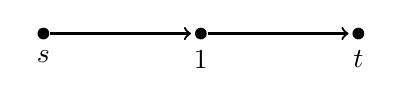
\begin{tikzpicture}[shorten >=1pt, thick]%[shorten >=1pt,node distance=2cm,>=stealth',thick]
  \node [shape=circle,fill=black,inner sep=1.5pt,label=below:$s$] (q0) at (0,0) {};
  \node [shape=circle,fill=black,inner sep=1.5pt,label=below:$1$] (q1) at (2,0) {};
  \node [shape=circle,fill=black,inner sep=1.5pt,label=below:$t$] (q2) at (4,0) {};
  \path[->] (q0) edge (q1) (q1) edge (q2);
\end{tikzpicture}
\end{center}
\caption[Grafo dirigido correspondiente a una estructura \A]{El grafo dirigido que corresponde a la estructura $\A=\tup{|\A|,E^\A,s^\A,t^\A}$
donde $|\A|=\{0,1,2\}$, $E^\A=\{(0,1),(1,2)\}$, $s^\A=0$ y $t^\A=2$.}
\label{grafo_simple}
\end{figure}

La siguiente definición será de utilidad para trabajar sobre la semántica
formal.
\begin{definition}
Sea $\A \in \struc[\sigma]$ y sea $i$ una función 
$i : \text{VAR}\ \deriv |\A|$, donde \text{VAR} es el conjunto de
todas las variables.
Se dice que el par $(\A, i)$ es una \textbf{interpretación} de una fórmula de
segundo orden $\Phi \in \LSO(\sigma)$.
\end{definition}
Como ejemplo, una posible interpretación de la fórmula $\Phi =
(\exists xy) (T(x, y))$
es $(\A, i)$, para toda variable $x$, donde $i(x) = 1$ y $\A$ es la estructura ejemplo mencionada
anteriormente.
\begin{definition}
Se extiende $i$ sobre todos los términos del lenguaje. Como no hay símbolos
funcionales, sólo es necesario extender $i$ sobre las constantes. Se define
$i(a) = a^\A$ para toda constante $a \in \sigma$.
\end{definition}

\subsection{Semántica formal}
Las definiciones \ref{semantica_def} y \ref{semantica_def2} describen 
bajo qué circunstancias una fórmula $\Phi$ en
$\LSO(\sigma)$ satisface una estructura $\A$, tal como es
presentado por \cite{immerman:book}.

\begin{definition}
\label{semantica_def}
\textbf{Definición de Verdad.} Sea $\A \in \struc[\sigma]$.
Se definen inductivamente las condiciones necesarias y suficientes para que 
una fórmula $\Phi \in \LSO(\sigma)$ sea verdadera bajo la interpretación $(\A, i)$:
\[
\begin{array}{lcl}
\text{(a)} \hspace{5mm} (\A, i) \models t_1 = t_2 & \iff & i(t_1) = i(t_2)\\
\text{(b)} \hspace{5mm} (\A, i) \models R(t_1,\ldots,t_{k}) & \iff & \tup{i(t_1),\ldots,i(t_{k})} \in R^{\A}\\
\text{(c)} \hspace{5mm} (\A, i) \models \neg \Phi & \iff & (A, i) \nvDash \Phi\\
\text{(d)} \hspace{5mm} (\A, i) \models \Phi \land \Psi & \iff & (\A, i) \models \Phi \mbox{ y } (\A, i) \models \Psi\\
\text{(e)} \hspace{5mm} (\A, i) \models \Phi \lor \Psi & \iff & (\A, i) \models \Phi \mbox{ o } (\A, i) \models \Psi\\
\text{(f)} \hspace{5mm} (\A, i) \models \Phi \Rightarrow \Psi & \iff & (\A, i) \models \neg \Phi \lor \Psi\\
\text{(g)} \hspace{5mm} (\A, i) \models (\exists x) \Phi & \iff & \mbox{existe } u \in |\A| 
\mbox{ tal que } (\A, i [x:= u]) \models \Phi,\\
&&\mbox{donde } i[x:=u](y) = \left\{
     \begin{array}{lr}
       u & \mbox{si } y = x\\
       i(y) & \mbox{si } y \not= x
     \end{array}
   \right.\\
\text{(h)} \hspace{5mm} (\A, i) \models (\forall x) \Phi & \iff &
    (\A, i) \nvDash (\exists x) \neg \Phi\\
\text{(i)} \hspace{5mm} (\A, i) \models (\exists R) \Phi & \iff & \mbox{existe } R' \subseteq |\A|^k
\mbox{ tal que } (\tup{\A, R'}, i) \models \Phi,\\
&&\text{donde } \tup{\A, R'} \text{ es la estructura que extiende a $\A$ }\\
&&\text{donde $R$ se interpreta como $R'$.}\\
\text{(j)} \hspace{5mm} (\A, i) \models (\forall R) \Phi & \iff &
    (\A, i) \nvDash (\exists R) \neg \Phi\\
\end{array}
\]
\end{definition}
\begin{definition}
\label{semantica_def2}
Se dice que $\A \models \Phi$ si y sólo si para toda función $i$ se cumple $(A, i)
\models \Phi$. Se dice que $\models \Phi$, o que $\Phi$ es verdadera, si y sólo si para
toda estructura $\A \in \struc(\sigma)$ se cumple $\A \models \Phi$.
\end{definition}

Volviendo al grafo de ejemplo \A, puede verificarse mediante semántica 
formal si $\A\models\Phi$, donde $\Phi$
es una fórmula arbitraria de $\LPO(\sigma)$. A continuación se comprueba si dos
fórmulas particulares satisfacen la estructura \A. 
%No se requiere utilizar la
%noción de interpretación, pues toda sentencia $\Phi \in LSO(\sigma)$ es
%verdadera o falsa en cualquier estructura $\A \in \struc[\sigma]$.

\begin{enumerate}
\item $\A\models^?(\exists x)(E(s,x)\land E(x,t))$

Sea $i : \text{VAR} \rightarrow |\A|$ arbitraria.\\
Considere $j = i[x:=1]$.\\
Se tiene por definición \ref{semantica_def}(b) que $(\A,j) \models E(s,1)$ y que $(\A,j) \models E(1,t)$.\\
$\tup{\text{por definición \ref{semantica_def}(d)}}$\\
\mbox{\hspace{5mm} $(\A,j) \models E(s,1)\ \land E(1,t)$}\\
$\iff \tup{\text{definición \ref{semantica_def}(g)}}$\\
\mbox{\hspace{5mm} $(\A,j) \models (\exists x)(E(s,x) \land E(x,t))$}\\
$\therefore\ \A \models \Phi$, porque $i$ es arbitraria.

%\item $\A\models^?(\exists R^1)(\forall x)(E(s,x) \land R(x))$
\item La sentencia
\[ \Phi_{\textsc{2Col}} = (\exists R^1)(\forall xy)(E(x,y)\Rightarrow \neg (R(x) \iff R(y))) \]
es cierta para un grafo si y sólo si es 2-coloreable. Se comprobará formalmente
que $\A \models \Phi_{\textsc{2Col}}$ y el grafo, por tanto, es 2-coloreable.

Sea $i : \text{VAR} \rightarrow |\A|$ arbitraria.\\
Considere $R' = \{1\}$, y sea $\tup{A, R'}$ la estructura que extiende a $\A$
donde $R$ se interpreta como $R'$.\\
Se tiene por definición \ref{semantica_def}(b) que $(\tup{\A, R'},i) 
\models E(0,1)$ y que \mbox{$(\tup{\A, R'},i) \models E(1,2)$}.\\
También se tiene que $(\tup{\A, R'}, i) \models R'(1)$, 
$(\tup{\A, R'}, i) \nvDash R'(0)$, y $(\tup{\A, R'}, i) \nvDash R'(1)$.\\
$\tup{\text{por definición \ref{semantica_def}(d) y (c)}}$\\
\mbox{\hspace{5mm} $(\tup{\A, R'}, i) \models E(0,1) \land E(1,2) \land \neg
R'(0) \land R'(1) \land \neg R'(2)$}\\
$\iff \tup{\text{operadores de la lógica proposicional}}$\\
\mbox{\hspace{5mm} $(\tup{\A, R'}, i) \models (E(0,1) \Rightarrow \neg R(0)
\iff R(1))\ \land$} \\ 
\mbox{\hspace{30mm} $(E(1,2) \Rightarrow R(1) \iff \neg R(2))$}\\
$\iff \tup{\text{definición \ref{semantica_def}(h)}}$\\
\mbox{\hspace{5mm} $(\tup{\A, R'}, i) 
\models (\forall xy)(E(x, y) \Rightarrow \neg(R'(x) \iff R'(y)))$}\\
$\iff \tup{\text{definición \ref{semantica_def}(i)}}$\\
\mbox{\hspace{5mm} $(\A, i) 
\models (\exists R^1)(\forall xy)(E(x, y) \Rightarrow \neg(R(x) \iff R(y)))$}\\
$\therefore\ \A \models \Phi$, porque $i$ es arbitraria.
\end{enumerate}

La Figura \ref{grafo_coloreado} muestra una 2-coloración del grafo correspondiente a \A
\ inducida por $R$.

\begin{figure}[h]
\begin{center}
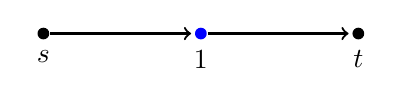
\begin{tikzpicture}[shorten >=1pt, thick]%[shorten >=1pt,node distance=2cm,>=stealth',thick]
  \node [shape=circle,fill=black,inner sep=1.5pt,label=below:$s$] (q0) at (0,0) {};
  \node [shape=circle,fill=blue,inner sep=1.5pt,label=below:$1$] (q1) at (2,0) {};
  \node [shape=circle,fill=black,inner sep=1.5pt,label=below:$t$] (q2) at (4,0) {};
  \path[->] (q0) edge (q1) (q1) edge (q2);
\end{tikzpicture}
\end{center}
\caption[Grafo dirigido coloreado por una relación]{El grafo dirigido de la Figura \ref{grafo_simple}, coloreado
utilizando la relación $R$. Los nodos para los cuales $R$ es verdadera son
azules, los otros son negros.}
\label{grafo_coloreado}
\end{figure}

\subsection{Abreviaciones sintácticas}
Con frecuencia es necesario cuantificar sobre una función de aridad $k$ ($f^k$)
en lugar de una relación. Esto puede hacerse cuantificando sobre una relación de
aridad $k+1$ ($F^{k+1}$) y agregando fórmulas de primer orden que garanticen
que $F$ represente a $f$. Por ejemplo, una función parcial unaria $f$ puede ser
representada por la relación binaria $F$ y la fórmula
\[ \psi_{fun} = (\forall xyy')(F(x, y) \land F(x, y') \Rightarrow y = y'). \]

De igual forma, se puede representar una función inyectiva añadiendo a las
proposiciones la fórmula anterior más

\[ \psi_{iny} = (\forall xx'y)(F(x, y) \land F(x', y) \Rightarrow x = x'). \]

Finalmente, si es necesario que la función sea total debe agregarse
\[ \psi_{tot} = (\forall x)(\exists y)(F(x, y)). \]

Se utilizarán las abreviaciones siguientes para denotar distintos
tipos de funciones:

\begin{tabular}{ll}
$(\exists F \in \text{Fun})$ & función total\\
$(\exists F \in \text{Inj})$ & función total inyectiva\\
$(\exists F \in \text{PFun})$ & función parcial\\
$(\exists F \in \text{PInj})$ & función parcial inyectiva\\
\end{tabular}

\subsection{Clases de complejidad}
El ejemplo anterior evidencia que una sentencia puede describir una colección
de estructuras discretas finitas (como grafos dirigidos) que satisfacen
una cierta propiedad (como 2-colorabilidad). 

En la TCD, un problema de decisión corresponde a una clase de estructuras de
primer orden que satisface a una sentencia, y por lo tanto los problemas de
decisión pueden ser \textbf{modelados con fórmulas lógicas de segundo orden}.
El trabajo de \cite{fagin:spectra} estableció que todos los problemas de
decisión en NP pueden ser caracterizados por la clase de estructuras que
satisfacen una sentencia de segundo orden existencial, es decir,
$\text{NP}=\SOE$.

Esta lista muestra los resultados más importantes de la TCD sobre la
caracterización de clases de complejidad \citep{immerman:book}:
\begin{itemize}
\item Espacio logarítmico no determinista (NL) es igual a la \LPO\ extendida con
un operador de clausura transitiva.
\item Espacio polinomial (P) es igual a las sentencias Horn de segundo orden
(SO-Horn).
\item Tiempo polinomial no determinista (NP) es igual a \SOE.
\item Co-NP es igual a \SOA.
\item La jerarquía de tiempo polinomial (PH) es igual a la lógica 
de segundo orden (\LSO) completa.
\item Espacio polinomial (PSPACE) es igual a la lógica de segundo orden
extendida con un operador de clausura transitiva.
\end{itemize}

%A transitive-closure operator is a \emph{syntactic construct}
%whose interpretation coincides with the transitive closure of
%a relation. Thus, it is not surprising that NL equals FO(TC)
%because checking the existence of a path from node $s$ to
%node $t$ in a digraph with designated vertices $s$ and $t$ is
%NL-complete \cite{sipser:book}, and this property
%holds whenever $s$ is related to $t$ in the transitive closure
%of the edge relation.

\section{Modelación de problemas}
\label{modelacionproblemas}
Consideremos, por ejemplo, el problema de satisfacibilidad
proposicional (SAT). Una instancia de SAT es una fórmula en forma normal
conjuntiva con $m$ cláusulas sobre $n$ variables proposicionales, donde una
cláusula es un subconjunto de literales positivos y negativos. 
Sean $P^2$, $N^2$ dos símbolos relacionales que describen las ocurrencias
positivas y negativas de los literales en las cláusulas: $P(x, y)$ expresa que
la variable $x$ aparece positiva en la cláusula $y$. Respectivamente, $N(x, y)$ expresa
su ocurrencia negativa.
Por ejemplo, $(p\lor \neg q\lor r)\land(\neg p\lor \neg r)\land(\neg p\lor q)$
es codificado como $\A=\tup{|\A|,N^\A,P^\A}$, donde $|\A|=\{0,1,2\}$,
$N^\A=\{(1,0),(0,1),(2,1),(0,2)\}$ y $P^\A=\{(0,0),(2,0),(1,2)\}$.

La existencia de una asignación de valores de verdad a las variables que
satisfaga una fórmula en forma normal conjuntiva (CNF) puede ser expresada con la
sentencia \SOE $\Phi_\SAT$:\footnote{Esta sentencia
asume que $m\geq n$. En caso contrario, se debe añadir cláusulas tautológicas a
la fórmula en CNF.}
\[ (\exists T^1)(\forall y)(\exists x)[(P(x,y)\land T(x))\lor(N(x,y)\land\neg T(x))] \]

La fórmula puede leerse como: existe una asignación de valores de verdad $T$
tal que en toda cláusula hay al menos una variable que cumple una de las
siguientes condiciones:
\begin{enumerate}[--]
\item la variable aparece positiva en la cláusula y está asignada a verdadero,
i.e. $T(x)$
\item la variable aparece negativa en la cláusula y está asignada a falso, i.e.
$\neg T(x)$
\end{enumerate}

Nótese que $T$ es un \textit{certificado}, pues muestra cuál es la asignación 
de variables necesaria para que la fórmula en CNF sea cierta.

En el Apéndice \ref{apendiceA} se encuentran las fórmulas correspondientes a
varios problemas NP, como camino hamiltoniano dirigido y colorabilidad de
grafos, entre otros.
